\section{Theory of Stellar Pulsations} 
\label{sec:pulsation}
\begin{shaded}
\noindent The purpose of this section is to give the reader a sufficient background summary on non-radial stellar pulsations in order to be able to understand the remainder of this thesis. 
I draw heavily here from the numerous textbooks that have been written on stellar pulsations, which include works by \cite{1926ics..book.....E}, \cite{1949ptvs.book.....R}, \cite{1979nos..book.....U}, \cite{1980tsp..book.....C}, \cite{2010aste.book.....a}, and \cite{basuchaplin2017}. 
Additionally, the long reviews by \cite{1958HDP....51..353L}, \citet{1993afd..conf..399G}, and \citet{2016lrsp...13....2b} were valuable references. 
I will perform calculations in this section using the \emph{Aarhus adiabatic oscillation package} \citep[\textsc{ADIPLS},][]{2008Ap&SS.316..113C}. 
\end{shaded}

Observations of stellar pulsations grant a new kind of insight into the behavior of stars. 
Whereas classical measurements of stars probe the stellar surface, observations of stellar pulsations, which traverse the stellar interior, bring deeper information to light. 
%shed light on the otherwise opaque stellar interior. %necessarily bring deeper information to light. 
Measurements of stellar pulsations provide stringent tests on the processes of stellar evolution, as the frequencies of pulsation profoundly depend on the predicted stellar structure. 
Stars exhibiting solar-like oscillations are particularly valuable for this pursuit. 
These stars vibrate in a superposition of a great number of oscillation modes simultaneously, and each mode that can be observed provides additional information that can be used to constrain stellar models. 

The pulsation hypothesis of stellar variability is supported by the fact that the theoretical pulsations of stellar models generally match the observed pulsations of stars. 
Furthermore, theoretically predicted pulsations in stars that were previously not observed to be variable (such as red giants) have been now overwhelmingly confirmed. 
That being said, while the agreement with models is very good, it is not perfect. 
%While the agreement with models very good, it is not perfect. 
In this section, I will outline the theory of stellar pulsations, thereby allowing us to calculate the time-independent adiabatic pulsation frequencies of our stellar models. 
I will compare the frequencies of my solar-calibrated model to measurements of the Sun. 
I will furthermore present the kernel functions of stellar structure, which quantify how changes to the stellar structure translate into changes in pulsation frequencies. 
This will allow me to state the structure inverse problem: i.e., the problem of determining a star's structure using only asteroseismic arguments. 
%In Chapter~\ref{chap:ML}, we will calculate the frequencies of many stellar models, and then try to determine the properties of observed stars by relating observations to the theory. 
%In Chapter~\ref{chap:statistical}, we will mine the models for patterns and quantify where the 



\subsubsection*{Assumptions} 

I again begin with my assumptions. In addition to the assumptions for stellar structure, I assume: 

\begin{enumerate} 
    \item \emph{The stellar structure is nearly static.} 
    I ignore all time derivatives (including velocities) in the equilibrium structure of the star. 
    Thus, I am considering only time-independent pulsation frequencies. 
    Clearly, stars evolve over time---the entire preceding section was based on that fact. 
    That said, the evolutionary timescale in the stars considered here (billions of years) is far greater than the pulsation timescale (minutes). 
    
    \item \emph{The pulsations are linear perturbations the static stellar structure.} 
    I ignore non-linear perturbations. %and all interactions. 
    This assumption should hold when the pulsation amplitudes are much smaller than the speed of sound. 
    As we've seen, solar oscillations have amplitudes around ${10\;\text{cm/s}}$, whereas the speed of sound at the surface of the solar-calibrated model is on the order of ${10\;\text{km/s}}$. 
    %This assumption breaks down in convection zones, where the interaction with convection damps the oscillations. 
    %We will deal with this drawback later in the section. 
    
    \item \emph{The pulsations are adiabatic.} 
    I ignore the transfer of energy between the oscillations and the equilibrium stellar structure. 
    This assumption should hold to good approximation when the pulsation time-scale is much smaller than the thermal timescale. 
    With pulsation periods on the order of minutes, this is true for the majority of the stellar interior.
    However, this assumption too breaks down near to the stellar surface. 
    Furthermore, without consideration of non-adiabatic effects, we will be unable to predict mode amplitudes, and we will not be able to determine whether the modes are excited \citep[e.g.,][]{2015EAS....73..111S}. 
    %Furthermore, this assumption prevents us from being able to theoretically predict mode amplitudes 
    %While  with the ability to predict amplitudes of stellar oscillations, nor whether an oscillation is excited. 
    %\item \emph{The pulsations do not interact with the stellar structure.} 
    %I treat the pulsations independently of time and ignore the interactions with convection. 
    %This assumption clearly breaks down in convection zones. 
    
    \item \emph{The stellar material is inviscid.} 
    I ignore internal friction. 
    Although the viscosity of the solar core is similar to that of honey (${\sim 100\;\text{cm}^2/\text{s}}$, e.g., \citealt{fox2000geophysical}), the Reynolds numbers throughout the solar interior are large enough to justify this assumption. %the viscosity timescale is much longer than the pulsation timescale. 
    %However, the neglected turbulent viscosity in convection zones may be important. 
    However, this assumption does break down in convection zones, where turbulent viscosity damps the oscillations. 
    %or even the lifetime of the Sun. 
\end{enumerate} 
Here and in the previous section I have made several assumptions that are violated in the near-surface layers of stars, or in locations where energy is transported by convection. 
These violations will cause errors in the predicted mode frequencies. 
I will introduce a correction to deal with these errors later in the section. 

\subsubsection*{Fluid Dynamics}
Given a static stellar structure, we consider a small perturbation that displaces all quantities (density, pressure, etc.) from equilibrium. %---density, pressure, and so on---from equilibrium by a displacement $\vec \xi$. 
For example, the stellar density at position $\vec r$ and time $t$ is 
\begin{align}
    \text{(Eulerian perturbation)} && 
    \rho (\vec r, t)
    &= \label{eq:eulerean}
    \rho_0 (\vec r) 
    + 
    \rho' (\vec r, t)
    \\
    \text{(Lagrangian perturbation)} &&
    \delta\rho(\vec r)
    &= \label{eq:lagrangian}
    \rho'(\vec r_0)
    +
    \vec\xi \cdot \nabla\rho_0 (\vec r)
\end{align}
where $\rho_0$ is the equilibrium density, $\rho'$ is the perturbed density, and ${\vec\xi\equiv\vec r - \vec r_0}$ is the displacement in space.
%Eulerian perturbations 
Here I have made use of the assumption that the equilibrium structure does not depend on time. 
The perturbation induces a velocity field $\vec{\varv}$ given by 
\begin{equation}
    \vec{\varv} (\vec r, t) 
    = 
    \frac{\partial}{\partial t}\vec\xi (\vec r, t).
\end{equation}
This velocity field is then controlled by the following equations: 
%the continuity equation, the equation of motion, the Poisson equation, and the heat equation. 
%I will again present these equations essentially without derivation. 
%I will at first give them in full 3D, and later apply symmetry arguments when appropriate. 

\begin{description}
    \setlength{\itemindent}{0pt}
    \item[The continuity equation.]
    As we've seen previously, the equation of continuity is a statement of mass conservation (\emph{cf}.~Equation~\ref{eq:cons-mass}). 
    It states that mass cannot teleport through the star, but rather must travel through it continuously. 
    \lr{The equation can be given as 
    \begin{equation} \label{eq:continuity} 
        \frac{\partial \rho}{\partial t}
        +
        \nabla
        \cdot
        \left(
            \rho \vec{\varv} 
        \right)
        =
        0
    \end{equation}
    where $\nabla\cdot$ is the divergence vector operator.} 
    Substituting the perturbed quantities (Equation~\ref{eq:eulerean}) into Equation~\ref{eq:continuity}, we get 
    \begin{equation}
        \frac{\partial}{\partial t} \left[
            \rho_0(\vec r)
            +
            \rho' (\vec r, t)
        \right]
        +
        \nabla\cdot \left\{
            \left[
                \rho_0(\vec r)
                +
                \rho'(\vec r, t)
            \right]
            \frac{\partial\vec\xi}{\partial t} 
        \right\}
        =
        0.
    \end{equation}
    %Since the equilibrium structure is static, the corresponding time derivatives vanish. 
    As we have assumed the equilibrium structure to be static, the corresponding time derivatives vanish. 
    Integrating with respect to time, we then obtain
    %The manipulation of this equation proceeds as follows. 
    %First, I substitute the quantities . 
    %Then, I drop the 
    %Substituting the displacement vector and Eulerian perturbations, dropping all time derivatives of the equilibrium quantities, dropping all interactions between perturbed quantities, we obtain
    \begin{equation} \label{eq:perturbed-continuity} \boxed{
        \rho' 
        + 
        \nabla \cdot \left( 
            \rho_0 \vec\xi 
        \right) 
        = 
        0
    }\end{equation}
    i.e., the perturbed equation of continuity. $\hfill\square\;$
    
    \item[The equation of motion.] \lr{To first order, the general Navier--Stokes momentum equation can be expressed as}
    \begin{equation} 
        \rho
        \left(
            \frac{\partial}{\partial t}
            +
            \vec{\varv}
            \cdot
            \nabla 
        \right)
        \vec{\varv}
        =
        -\nabla P
        +
        \mu \nabla^2 \vec{\varv}
        +
        \frac{1}{3} \mu \nabla\left(
            \nabla \cdot \vec{\varv}
        \right)
        +
        \rho \vec{g}
    \end{equation}
    where $\mu$ is the viscosity of the stellar material and $\vec{g}$ is the gravitational acceleration.
    Since I have assumed that the stellar viscosity is negligible, we can obtain 
    \begin{equation} \label{eq:momentum} %\boxed{
        \rho
        \left(
            \frac{\partial}{\partial t}
            +
            \vec{\varv}
            \cdot
            \nabla 
        \right)
        \vec{\varv}
        =
        -
        \nabla P
        +
        \rho \vec g%\nabla \Phi.
    \end{equation}
    Notice that this equation at equilibrium is the familiar equation of hydrostatic support (\ref{eq:cons-mom-r}):
    \lr{\begin{equation}
        0 = -\nabla P_0 + \rho_0 \vec{g}_0.
    \end{equation}}
    %We may now substitute in Equation~(\ref{eq:momentum}) the gravitational acceleration for the gradient of the gravitational potential:
    Substituting the perturbations into Equation~(\ref{eq:momentum}) and dropping all higher-order terms, we find the perturbed equation of motion:
    \lr{\begin{equation} \label{eq:perturbed-motion} \boxed{
        \rho_0\,
        \frac{\partial^2 \vec\xi}{\partial t^2}
        =
        -\nabla P'
        -
        \rho_0 \nabla \Phi'
        -
        \rho' \nabla \Phi_0
    }\,.\end{equation}
    Here I have introduced the gravitational potential $\Phi$, the negative gradient of which is the gravitational acceleration: %, i.e., the gradient of the gravitational acceleration: 
    \begin{equation} \label{eq:grav-pot}
        \vec g 
        =
        - \nabla \Phi
        \qquad
        \text{and}
        \qquad
        \Phi(\vec r, t)
        =
        -G
        \int_{V}
            \frac{\rho}{|\vec r - \vec x|}
        \;\text{d}^3 \vec{x}
    \end{equation}
    where $V$ is the volume of the star at equilibrium.} 
    %and then we find the perturbed equation of motion:
    %where $\mathbf{\Phi}$ is the gravitational potential. 
    
    \item[Poisson's equation.] %We may supplement these equations with a relation between the stellar structure and the gravitational field. 
    Gauss's law for gravity gives that
    \begin{equation}
        \nabla \cdot \vec g
        =
        -4\pi G \rho.
    \end{equation}
    After substituting the gravitational potential and the Eulerian perturbations, we obtain the perturbed Poisson equation to describe the gravitational field: 
    %\begin{equation} \label{eq:poisson} %\boxed{
    %    \nabla^2 \Phi = 4\pi G \rho. 
    %\end{equation} 
    %After substitution, we find
    \begin{equation} \label{eq:perturbed-poisson} \boxed{
        \nabla^2 \Phi'
        =
        4\pi G \rho'
    }\,.\end{equation}
    
    \item[The energy equation.]
    The energy equation completes the system by thermodynamically connecting pressure to density. 
    Since I have assumed adiabatic pulsations, the energy equation can be given as
    \begin{equation} %\boxed{
        \frac{\partial P}{\partial t}
        +
        \vec{\varv}
        \cdot
        \nabla P
        =
        c^2 
        \left(
            \frac{\partial \rho}{\partial t}
            +
            \vec{\varv} \cdot \nabla \rho
        \right)
    \end{equation}
    where $c$ is again the adiabatic speed of sound (\emph{cf.}~Equation~\ref{eq:speed-of-sound}). 
    Substituting the Lagrangian perturbation, we obtain the perturbed energy equation
    \begin{equation} \label{eq:perturbed-energy} \boxed{
        P'
        +
        \vec \xi \cdot \nabla P_0
        =
        c^2_0 \left( 
            \rho' + \vec \xi \cdot \nabla \rho_0
        \right)
    }\,.\end{equation}
\end{description}


\subsubsection*{Symmetry}
Now I will apply the assumption of symmetry and consider only oscillatory solutions on a sphere. 
\lr{I separate the displacement vector into radial and horizontal components 
%${\vec\xi = \xi_r \hat a_r + \vec \xi_h}$, ${\vec\xi_h = \xi_\theta \hat a_\theta + \xi_\phi \hat a_\phi}$, 
\begin{equation}
    \vec\xi = \xi_r \hat a_r + \vec \xi_h, 
    \qquad 
    \vec\xi_h = \xi_\theta \hat a_\theta + \xi_\phi \hat a_\phi
\end{equation}
where $\hat a$ are unit vectors in indicated directions. 
%${\vec\xi\equiv[\xi_r, \xi_h]}$.
The radial component of the displacement, for example, can now be expressed as
%The radial displacement, for example, can be now expressed as 
\begin{align}
    \xi_r(r, \theta, \phi, t)
    &=
    \xi_r(r)
    Y_{\ell}(\theta, \phi)
    \exp \{
        -i\omega t
    \} %\vphantom{\Bigg\{}
\end{align}
where $\theta$ and $\phi$ are latitude and longitude, $Y_{\ell}$ is Laplace's spherical harmonic for degree $\ell$ (\emph{cf.}~Figure~\ref{fig:sph}), $i$ is the imaginary unit, and ${\omega=2\pi\nu}$ is the cyclic frequency.}
When $\omega^2$ is real, the solution is oscillatory; when it is imaginary, the solution either grows or delays. 
Substituting the spherical, symmetric, harmonic variables into the previous equations (\ref{eq:perturbed-continuity}, \ref{eq:perturbed-motion}, \ref{eq:perturbed-poisson}, \ref{eq:perturbed-energy}) and dropping subscripts for unperturbed quantities, after some manipulations we may find 
\begin{gather} \label{eq:oscillation1}
    \frac{\text{d}\xi_r}{\text{d}r}
    =
    -\left(
        \frac{2}{r}
        +
        \frac{1}{\Gamma_1 P}
        \frac{\text{d}P}{\text{d}r}
    \right)
    \xi_r
    +
    \frac{1}{\rho c^2}
    \left(
        \frac{S_\ell^2}{\omega^2}
        -
        1
    \right)
    P'
    -
    \frac{\ell(\ell+1)}{\omega^2 r^2}
    \Phi' \vphantom{\Bigg(}
    \\
    \frac{\text{d}P'}{\text{d}r}
    =
    \rho \left(
        \omega^2 - N^2
    \right) 
    \xi_r
    +
    \frac{1}{\Gamma_1 P}
    \frac{\text{d}P}{\text{d}r}
    P'
    +
    \rho \frac{\text{d} \Phi'}{\text{d} r}
    \vphantom{\Bigg(}
    \\
    \frac{1}{r^2}
    \frac{\text{d}}{\text{d}r}
    \left(
        r^2\,
        \frac{\text{d}\Phi'}{\text{d}r}
    \right)
    =
    -4\pi G \left(
        \frac{P'}{c^2}
        +
        \frac{\rho}{g}
        \xi_r
        N^2
    \right)
    +
    \frac{\ell(\ell+1)}{r^2}
    \Phi' \vphantom{\Bigg(}
    \label{eq:oscillation3}
    %\\
    %\xi_h(r)
    %&=\label{eq:oscillation3}
\end{gather}%
\lr{as well as 
\begin{gather}
    \vec\xi_h(r, \theta, \phi, t) 
    =
    \sqrt{4\pi}\,
    \xi_h(r)
    %\frac{\sqrt{4\pi}}{r\omega^2} \left( 
    %    \frac{P'}{\rho} - \Phi'
    %\right)
    \left(
        \frac{\partial Y_\ell}{\partial \theta}\,
        \hat{a}_\theta
        +
        \frac{1}{\sin\theta}
        \frac{\partial Y_\ell}{\partial \phi}\,
        \hat{a}_\phi
    \right)
    \exp \{
        -i\omega t
    \} \vphantom{\Bigg(}
    \\
    \xi_h(r)
    =
    \frac{1}{r\omega^2} \left( 
        \frac{1}{\rho}\, P' - \Phi'
    \right). \vphantom{\Bigg(}
\end{gather}}
%where $\hat a$ are unit vectors in the indicated directions. 
Here I have introduced the \emph{Brunt-V\"ais\"al\"a} and \emph{Lamb} \lr{squared} frequencies: 
\begin{gather} \label{eq:brunt-vaisala}
%\begin{aligned}
    N^2
    =
    g
    \left(
        \frac{1}{\Gamma_1}
        \frac{\text{d} \ln P}{\text{d}r}
        -
        \frac{\text{d} \ln \rho}{\text{d}r}
    \right) 
    \\ \label{eq:lamb}
    S^2_\ell
    =
    \frac{\ell(\ell+1)c^2}{r^2}
%\end{aligned}
\end{gather}
which give the regions in the star where modes of different character can propagate. 
The former, $N^2$, describes where g-modes can propagate, so called because their restoring force is gravity. 
The latter, $S_\ell^2$, depending on the spherical degree $\ell$, describes where p-modes can propagate, called as such because their restoring force is the pressure gradient. 
These cavities are visualized in Figure~\ref{fig:propagation}. 
%g-modes---modes whose restoring force are gravity---and p-modes---modes whose restoring force is the pressure gradient---can propagate, respectively . 
Here it can be appreciated that g-modes and convection are two sides of the same coin: when ${N^2<0}$ the fluid is unstable to convection; otherwise, the fluid is unstable to g-mode oscillations. 

This system of equations (\ref{eq:oscillation1}--\ref{eq:oscillation3}) constitutes a fourth order boundary eigenvalue problem. 
Equipped with suitable boundary conditions, we may numerically calculate the eigenfunctions $\vec\xi$ (see Figure~\ref{fig:eigenfunctions}) and their corresponding eigenfrequencies $\omega$ for a given model of stellar structure. 
This is the forward problem of stellar pulsation. 


\begin{figure}
    \centering
    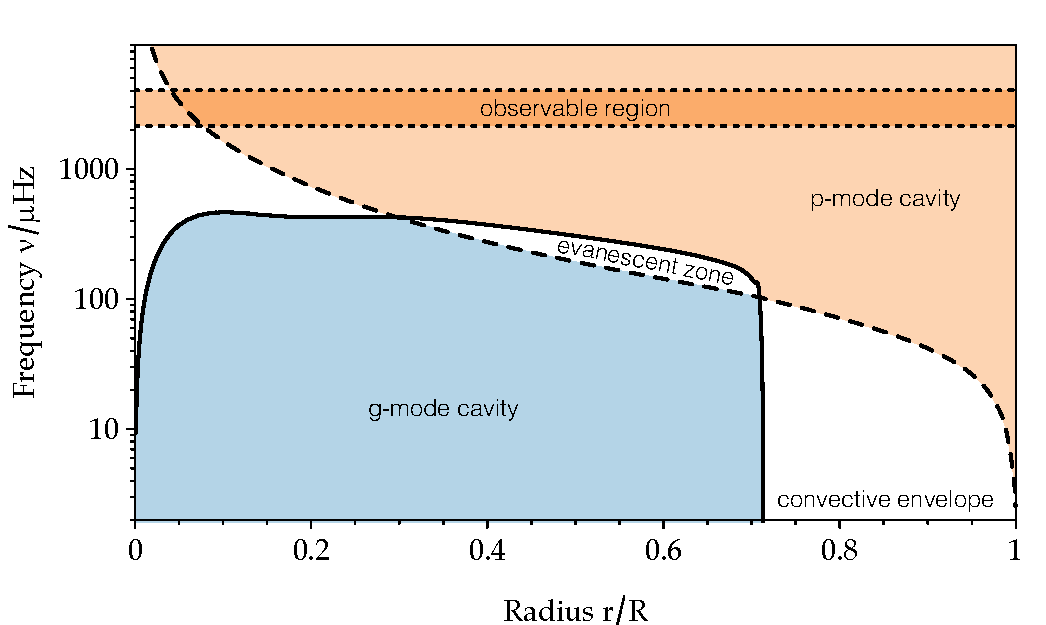
\includegraphics[width=\textwidth]{ch1_introduction/figs/pulse/prop-solar.pdf}
    \caption[Propagation diagram]{Propagation diagram for a solar model. 
    The blue-shaded area shows the Brunt-V\"ais\"al\"a region where g-modes can propagate (\emph{cf.}~Equation~\ref{eq:brunt-vaisala}). 
    %The Brunt-V\"ais\"al\"a frequency becomes imaginary in convective zones. 
    The orange-shaded area shows the ${\ell=1}$ Lamb region where dipolar p-modes can propagate (\emph{cf.}~Equation~\ref{eq:lamb}). 
    Modes are exponentially damped in the evanescent zone; nevertheless, modes of similar frequency can couple in this region, giving rise to mixed modes. 
    The observable region is a few ${\Delta\nu}$ around $\nu_{\max}$; thus, only p-modes are expected to be observed in this range at this stage of evolution. 
    \label{fig:propagation}}
\end{figure}

%\subsubsection*{Boundary Conditions}


%\subsubsection*{Numerical Solutions}

\begin{figure}
    \centering
    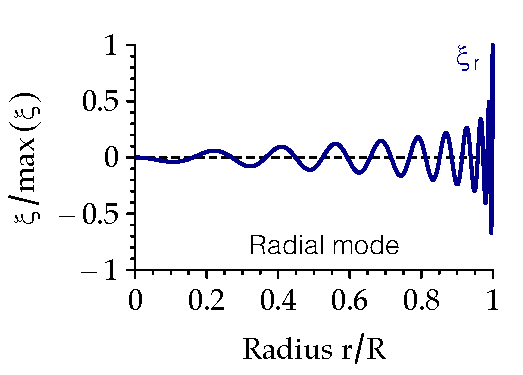
\includegraphics[width=0.5\textwidth]{figs/pulse/eig-radial.pdf}%
    \makebox[0.5\textwidth][c]{%
        \adjustbox{trim={1.7cm 0cm 0cm 0cm},clip}{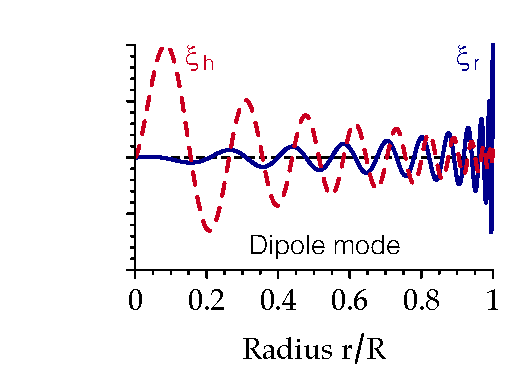
\includegraphics[width=0.5\textwidth]{figs/pulse/eig-dipole.pdf}}}
    \caption[Eigenfunctions]{Radial (blue) and horizontal (red) normalized eigenfunctions for radial (${\ell=0}$, left) and dipolar (${\ell=1}$, right) oscillation modes, both having radial order ${n=20}$. 
    The radial displacement of the two modes are quite similar, being only slightly offset in the interior and basically identical in the envelope. 
    The horizontal displacement has zero crossings when the radial displacement is maximal, and vice versa. 
    Radial modes lack horizontal displacement by definition. 
    \label{fig:eigenfunctions}}
\end{figure}



\subsubsection*{Some Properties of Solar-like Oscillations}

As we have seen in the first section, oscillation modes of the same spherical degree $\ell$ can differ in their radial order $n$ and be excited simultaneously with different frequencies. 
For solar-type stars, it is currently possible to resolve frequencies for modes of low spherical degree (${0~\leq~\ell~\leq~3}$) and `high' radial order (${8~\leq~n~\leq~31}$). 
The frequency range where oscillation power is maximum, called by $\nu_{\max}$, generally corresponds to around ${n=20}$ or so. 
This region of power is proportional to (and obviously lower than) the acoustic cut-off frequency, i.e., the upper frequency bound for oscillations to be reflected back into the star rather than being lost to space: 
\begin{equation} \label{eq:numax}
    \nu_{\max} \propto \nu_{\text{ac}} \propto \frac{g}{\sqrt{T_{\text{eff}}}}.  %\frac{g}{\sqrt{T_{\text{eff}}}}
    %g\sqrt{\frac{\mu}{T}}%{\sqrt{T_{\text{eff}}}}
\end{equation}
For the Sun, ${\nu_{\max,\odot} \simeq 3090\;\mu\text{Hz}}$ (${\sim 5.4}$~minutes) and ${\nu_{\text{ac},\odot} \simeq 5000\;\mu\text{Hz}}$ (${\sim 3.3}$~minutes). 
Since we lack a proper theoretical treatment of convective transport, which both excites and damps the oscillation modes, we are unable to theoretically predict the amplitudes of the oscillations of our solar model. 
In lieu of this, we may try to predict the general region where oscillations with the greatest amplitudes are to be expected by scaling from the observed solar values \citep[e.g.,][]{1995A&A...293...87K}:
\begin{equation}
    \frac{\nu_{\max,\ast}}{\nu_{\max,\odot}}
    =
    \left(
        \frac{M_\ast}{M_\odot}
    \right)
    \left(
        \frac{R_\ast}{R_\odot}
    \right)^{-2}
    \left(
        \frac{T_{\text{eff},\ast}}{T_{\text{eff},\odot}}
    \right)^{-\frac{1}{2}}
    %\left(
    %    \frac{\mu_\ast}{\mu_\odot}
    %\right)^{\frac{1}{2}}
\end{equation}
and likewise for the acoustic cutoff frequency. 
%We cannot calculate these quantities for our solar models because we have assumed adiabatic oscillations and have therefore lost any information about mode amplitudes.
%This equation will later help give us a practical first-order solution to our inverse problem. 

\citet{1980ApJS...43..469T} considered oscillation modes in the asymptotic limit of high radial order (${n\gg\ell}$) and found that theoretical mode frequencies form a pattern. 
In particular, adjacent modes of the same spherical degree are approximately equally spaced, which agrees with the observations that we saw in Figures~\ref{fig:solar-power-spectrum} and \ref{fig:16cygb}. 
The pattern of frequencies can be summarized to first-order approximation as 
\begin{equation} \label{eq:asymptotic}
    \nu_{n,\ell} \simeq \Delta\nu \left( n + \frac{\ell}{2} + \epsilon \right)
\end{equation}
where $\nu_{n,\ell}$ is the frequency of mode (${n,\ell}$) and $\epsilon$ is a phase shift (${\epsilon_\odot\simeq 1.6}$). 
The spacing ${\Delta\nu}$ is called the \emph{large frequency separation} and is related to the inverse sound travel time and proportional to the \lr{root mean density} of the star \citep{1986apj...306l..37u, 1995A&A...293...87K}:
\begin{equation}
    \Delta\nu
    \simeq
    \left( 
        2 \int \frac{\text{d}r}{c}
    \right)^{-1}
    \propto
    \left(
        \frac{M}{R^3}
    \right)^{1/2}. 
    %\sqrt{\bar{\rho}}
    %\qquad\text{and}\qquad
    %\Delta\nu 
\end{equation}
Since the large frequency separation gives the spacing between modes of different orders, it can be calculated empirically with
\begin{equation} \label{eq:Dnu}
    \Delta\nu_{n,\ell} 
    =
    \nu_{n,\ell}
    -
    \nu_{n-1,\ell}.
\end{equation}
Calculating the average large frequency separation of the Sun for radial modes using data from the Birmingham Solar Oscillations Network \citep[\emph{BiSON},][]{2009mnras.396l.100b} we can obtain 
\begin{equation}
    \Delta\nu_\odot = 134.8693 \pm 0.0042\;\mu\text{Hz}. 
\end{equation}
%The large frequency separation has the interesting properties that it is proportional to the stellar root mean density and approximately equal to the inverse sound travel time: 
%Later we will see that $\Delta\nu$ and $\nu_{\max}$ give a practical and widely-used first-order solution to our inverse problem. 
This presents an opportunity to test the quality of our solar model. 
We can calculate the large frequency for our solar-calibrated model either using the inverse sound travel time, or using the frequencies themselves. 
In the former case, we obtain ${\Delta\nu = 136.2970\;\mu\text{Hz}}$. 
In the latter, ${\Delta\nu = 136.2208\;\mu\text{Hz}}$. 

On the one hand, these model values differ by only about one percent from the solar values, which is quite good by astrophysical standards. 
On the other hand, when considering the precision with which ${\Delta\nu_{\odot}}$ can be calculated, this is a highly significant ${\sim 300\sigma}$ difference. 
This difference arises due to our ill treatment of the stellar surface, which we will address later in this section. 

%The quantity $\Delta\nu$ is the \emph{large frequency separation}---the spacing between consecutive radial mode frequencies. %---which turns out to be proportional to the stellar mean density and approximately equal to the inverse sound travel time through the star:
A higher-order expansion of the asymptotic expression additionally gives a term known as the \emph{small frequency separation}, the spacing between modes adjacent in frequency and whose spherical degree differs by two \lr{\citep{1980ApJS...43..469T}}: 
\begin{equation} \label{eq:dnu}
    \delta\nu_{n,\ell}
    =
    \nu_{n,\ell}
    -
    \nu_{n-1,\ell+2}
    \simeq
    -(4\ell + 6)
    \frac{\Delta\nu}{4\pi^2 \nu_{n,\ell}}
    \int
        \frac{\text{d}c}{\text{d}r}
        \frac{\text{d}r}{r}.
\end{equation}
As we can see, the small frequency separation is sensitive to the sound speed gradient, and is therefore a good proxy for the conditions in the stellar core, where the sound speed gradient changes sign (\emph{cf.}~Figure~\ref{fig:profs}). 
This makes ${\delta\nu}$ a diagnostic of main-sequence age. 
%This term can also be calculated from the observations: 
We will make use of these relations to infer the properties of stars in Chapter~\ref{chap:ML}, and use computational methods to further understand what properties of stars they reflect in Chapter~\ref{chap:statistical}. 
The average small frequency separation between solar oscillation modes with (${\ell=0},\;{\ell=2}$) is
\begin{equation}
    \delta\nu_\odot \simeq 8.957 \pm 0.059\;\mu\text{Hz}
\end{equation}
and for our solar model, ${\delta\nu=8.939\;\mu\text{Hz}}$, which is good agreement. 
%Asymptotically, the small frequency separation can be given as 
%\begin{equation} 
%\end{equation}
%For our solar model, the asymptotic small frequency separation is $\delta\nu = $ 8.939086\;\mu\text{Hz}$, and from the calculated adiabatic pulsation frequencies,. 



\subsubsection*{A Direct Comparison} 
We have just compared our solar model against the asymptotic properties of the solar oscillations, finding good agreement with the small frequency separation but less good agreement with the large frequency separation. 
We may now test the quality of our solar model more directly by comparing the individual pulsation mode frequencies themselves to those observed in the Sun. 
This comparison is shown in Figure~\ref{fig:solar_freq_diffs}. 
%Figure~\ref{fig:solar_freq_diffs} shows this comparison by relative differences $\delta\nu/\nu$. 

Immediately it can be seen that there are systematic discrepancies between the model and the actual mode frequencies on the order of ${10\;\mu\text{Hz}}$, i.e., tenths of a percent, which is a difference in period of about $1$ to $2$ seconds. 
In particular, the disagreement gets worse with increasing frequency. 
This phenomenon is called the \emph{surface effect} and has arisen from our improper modelling of the near-surface layers \citep[e.g.,][]{1984srps.conf...11C}. 
The large frequency separation is also sensitive to surface effects, which is why our model ${\Delta\nu}$ differed so significantly from the observed value. 

It is noteworthy that, because all of the waves propagate essentially radially in the near-surface layers (\emph{cf.}~Figures~\ref{fig:rays} and \ref{fig:eigenfunctions}), the surface term is a function of frequency alone and is independent of the spherical degrees of the modes. 
The surface effect is thus often dealt with by introducing a correction that increases with frequency. %which is a function of frequency and normalized by the mode inertia. 
%\citet{1990LNP...367..283G} argued that the surface term should have a 
The \citet{2014A&A...568A.123B} treatment of the surface term fits coefficients $\mathbf a$ to the differences between observed and model frequencies according to
\begin{equation} \label{eq:BallGizon-surfterm}
    \delta \nu_{n,\ell} 
    = 
    \frac{1}{I_{n,\ell}} \left[ 
        a_1 \left( 
            \frac{\nu_{n,\ell}}{\nu_{ac}} 
        \right)^{-1} 
        + 
        a_2 \left( 
            \frac{\nu_{n,\ell}}{\nu_{ac}} 
        \right)^{3} 
    \right] %\\
    %\Rightarrow F(\nu_i) = \frac{\delta \nu_i}{\nu_i} &= a \left( \frac{\nu_i}{\nu_{ac}} \right)^{-2} + b \left( \frac{\nu_i}{\nu_{ac}} \right)^{2}
\end{equation}
where $\nu_{ac}$ is the acoustic cutoff frequency, with ${\nu_{ac,\odot} \approx 5000}$, and $I_{n,\ell}$ is the normalized mode inertia:
\begin{equation} \label{eq:normalized-mode-inertia}
    I_{n,\ell}
    =
    \frac{4\pi}{M}
    \frac{\int \rho
            \left(
                |\xi_r|^2
                +
                \Ltwo |\xi_h|^2
            \right) 
            r^2
        \;\text{d}r}{
            |\xi_r(r=R)|^2
            +
            \Ltwo
            |\xi_h(r=R)|^2
        }.
\end{equation}
However, Figure~\ref{fig:solar_freq_diffs} further shows that even after correcting for the surface term, differences remain. 
This implies that even beyond the near-surface layers, the structure of the Sun differs from the model. 

\begin{figure}[t]
    \centering
    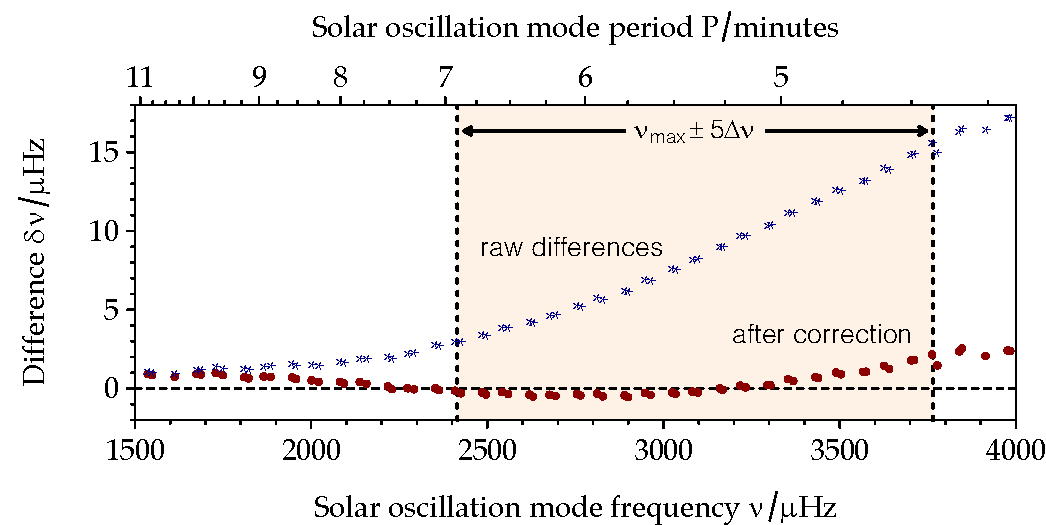
\includegraphics[width=\textwidth,keepaspectratio,trim={0cm 0cm 0cm 0.1cm}, clip]{figs/pulse/freq-diffs-solar.pdf}%solar_freq_diffs-hlD.pdf} 
    \caption[The solar surface effect]{Differences in oscillation frequencies between the Sun and the best-fitting solar model, in the sense of (model $-$ Sun). 
    Even after correcting for the surface term, substantial differences remain. 
    Being that solar frequencies are measured on the order of one part in a thousand, the uncertainties are too small to be visible at this resolution. 
    The offset at zero is likely due to the assumed solar radius differing from the helioseismic radius. 
    The shaded region indicates what the frequency range of the Sun might be if it were a field star observed by \emph{Kepler}. 
    \label{fig:solar_freq_diffs}} 
\end{figure} 

This motivates the inverse approach. 
We have seen that evolutionary theory can produce a model that agrees with the overall properties of the Sun. 
However, a detailed inspection of the mode frequencies of the model reveals significant disagreement between theory and observation, even after applying corrections. 
We wish to deduce the actual structure of the Sun and the stars using only asteroseismic arguments: i.e., to find the structure that will pulsate identically. 
This problem of deducing the structure of a star from its oscillation frequencies is inverse to the problem of deducing the oscillation frequencies from a given stellar structure. 
In order to pose the inverse problem in a manner that we can solve, however, it is convenient to first make some slight adjustments to our statement of the respective forward problem. 

%By considering the structure of the stellar model until it agrees with the observed oscillation mode frequencies, helioseismic and asteroseismic inversions allow the actual structure of the Sun (or the star under investigation) to be revealed, and be revealed in a way that is independent of the theory of stellar evolution. 


\subsection{The Relative Forward Problem} \label{sec:variational}
The forward problem of asteroseismology is to calculate the seismic frequencies of a stellar model. 
However, it is not clear how one would go about solving the inverse problem corresponding to this forward problem. 
Instead, we restate the forward problem as the problem of calculating the frequency \emph{differences} with respect to another model---one with a different structure. 
That is: by comparing the differences in structure of two models, what will be the differences in their frequencies? 
I call this the relative forward problem of asteroseismology. 
%Later, we will solve the corresponding inverse problem, that is: by comparing the differences in frequencies, what is the difference in structure? 

The benefit of posing the problem in this way is that it facilitates the inverse problem, which is to ask: by comparing the frequencies of the two models, what is the difference in their structure? 
Thus, since we are able to observe frequencies of real stars, we may substitute a star for one of the models, and hence measure the structure of a star. 
%This formulation facilitates an inverse problem 

To give a concrete example, I have calibrated another solar model using different assumptions on the physics of the stellar interior. 
In particular, this second model differs in that it does not include the effects of elemental diffusion and gravitational settling (i.e., $\mathbf{D}$ is the null matrix in Equation~\ref{eq:evol-diffusion}). 
This model has the same mass, radius, luminosity, metallicity, and age as the diffusion model---yet it differs in internal structure (see Figure~\ref{fig:prof_diffs}). %. shows the relative differences in internal structure between these two models of the Sun. %isothermal sound speed $u$, density $\rho$, the first adiabatic exponent $\Gamma_1$, and helium abundance $Y$ between these two models of the Sun. 
The differences in internal structure then give rise to differences in oscillation mode frequencies. %, and the kernel functions quantify that response. 

In order to state the relative forward problem, I will first put the oscillation equations in their so-called \emph{variational formulation}, and then %, which requires the assumption of the zero-boundary conditions. 
linearize the variational frequencies around a reference model. 
%It requires us to linearize the equations around a given reference model, and also new boundary conditions. 
The end result will be a Fredholm integral equation relating the relative differences in oscillation mode frequencies to the relative differences in structure, which will then be a suitable starting point for the inverse analysis. 


\begin{figure}
    \centering
    \begin{subfigure}[b]{0.5\linewidth}
        \centering
        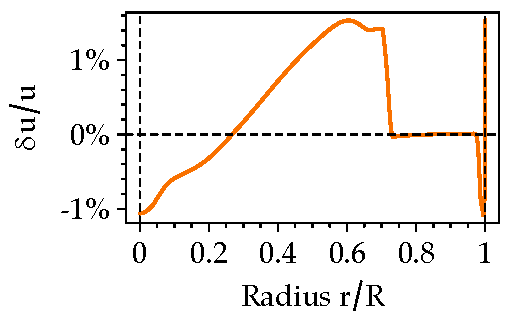
\includegraphics[width=\textwidth,keepaspectratio]{figs/pulse/diffs/d_u-D_no_diffusion.pdf}
    \end{subfigure}%
    \begin{subfigure}[b]{0.5\linewidth}
        \centering
        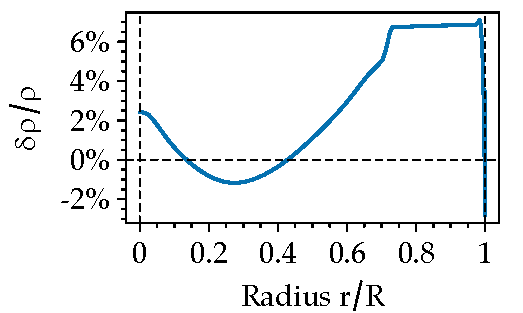
\includegraphics[width=\textwidth,keepaspectratio]{figs/pulse/diffs/d_rho-D_no_diffusion.pdf}%d_rho-D_noD.pdf}
    \end{subfigure}\\
    \begin{subfigure}[b]{0.5\linewidth}
        \centering
        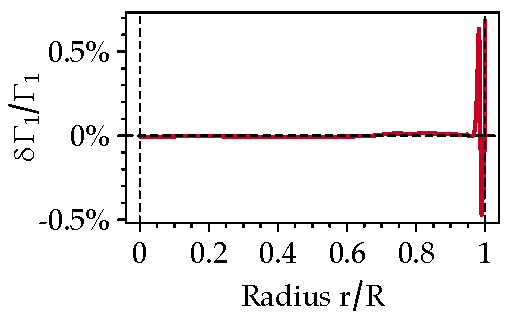
\includegraphics[width=\textwidth,keepaspectratio]{figs/pulse/diffs/d_Gamma1-D_no_diffusion.pdf}%d_Gamma1-D_noD.pdf}
    \end{subfigure}%
    \begin{subfigure}[b]{0.5\linewidth}
        \centering
        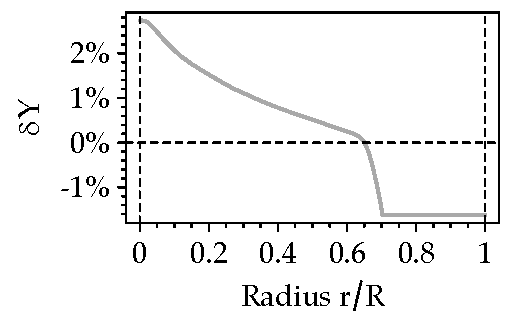
\includegraphics[width=\textwidth,keepaspectratio]{figs/pulse/diffs/d_Y-D_no_diffusion.pdf}%d_Y-D_noD.pdf}
    \end{subfigure}
    \caption[Structural differences between two solar models]{Relative differences in isothermal sound speed (top left), density (top right), the first adiabatic exponent (bottom left), and helium abundance (bottom right) as a function of radius between two solar-calibrated models with differing input physics (\emph{cf}.~Figure~\ref{fig:profs}). 
    %Differences are in the sense of (diffusive model minus non-diffusive model)/(diffusive model), except in the case of $Y$, which is absent of the denominator.  
    Although the models have the same overall properties (e.g.\ mass \& age); they differ structurally and chemically throughout their interiors. %The only exception to this is $\Gamma_1$, which is very near to 5/3 in the interiors of both models and differs mainly in the near-surface layers.
    %\emph{\textbf{TODO}: remake figures}
    } 
    \label{fig:prof_diffs} 
\end{figure}



%The theory of stellar evolution allows us to obtain best-. 
%However, the oscillation modes of the best model may still differ from the observed star. We know this to be the case for example with the Sun: although models of the Sun are quite good---in the sense that a model of the Sun obtained through evolutionary calibration can reproduce the correct mass, radius, luminosity, and so on---no evolutionary solar model has so far been able to exactly match the pulsation frequencies of the Sun. 

%As we have seen, the mode frequencies of our best-fitting solar model do not match those of the Sun. 
%Differences remain even after correcting for the surface term. 

\subsubsection*{Variational Frequencies}
%It is not straightforward to cast the oscillation equations in the relative forward  % a form that is suitable for the inverse analysis. 
%The left-hand side of the perturbed equation of motion (\ref{eq:perturbed-motion}) features the second derivative of the displacement vector. 
The perturbed hydrodynamical equations  (\ref{eq:oscillation1}--\ref{eq:oscillation3}) feature derivatives of the displacement vector. 
%If we seek only periodic solutions, then we obtain 
Since we have sought only periodic solutions, we have
\lr{\begin{equation}
    \vec\xi(t)
    =
    \vec\xi\cdot\exp\{i\omega t\}
    \qquad \Rightarrow \qquad
    \frac{\partial\vec\xi}{\partial t}
    =
    -i\omega\vec\xi.
    %\rho \frac{\delta^2 \vec\xi}{\delta t^2}
    %=
    %-\omega^2 \rho \vec\xi. 
\end{equation}}
Combining the perturbed equations, we can arrive at \citep[e.g.,][]{1979nos..book.....U}
\lr{\begin{equation} \label{eq:first-omega}
    -\omega^2 \rho \vec\xi
    =
    \nabla \left(
        c^2 \rho \nabla \cdot \vec \xi
        +
        \nabla P \cdot \vec \xi
    \right)
    -
    \vec g \,
    %\left[ 
        \nabla \cdot \left(
            \rho \vec \xi 
        \right)
    %\right]
    +
    \rho \vec g' %\nabla \Phi'
\end{equation}}
where I have dropped the subscripts on the unperturbed quantities. 
This equation relates the cyclic frequency $\omega$ to the properties of the stellar structure. 
Recalling Equation~(\ref{eq:grav-pot}), we can substitute the perturbed gravitational potential with 
\lr{\begin{equation}
    \vec g'
    =
    -\nabla \Phi'
    =
    G \nabla
    \int_V
        \frac{\rho'}{|\vec r - \vec x|}%\vec r - \vec r'|}
        %\nabla \cdot \left(\rho \vec \xi \right)
    \;\text{d}^3 \vec{x}
    =
    -G \nabla \int_V
        \frac{\nabla%_{\vec x}
            \cdot \left(
                \rho%(\vec x)
                \vec\xi%(\vec x)
            \right)}{|\vec r - \vec x|}%\vec r - \vec r'|}
    \;\text{d}^3 \vec{x}.
\end{equation}}
where the latter substitution makes use of the perturbed equation of continuity (Equation~\ref{eq:perturbed-continuity}). 
%where $V$ is the equilibrium volume of the star. 
%Now assuming 
%where I have assumed in the latter substitution that ${\rho(r=R)=0}$, i.e., the zero-boundary condition. %, we may obtain
%\begin{equation}
%
%\end{equation}
Thus, all terms in the right hand side of Equation~(\ref{eq:first-omega}) are functions of $\vec\xi$, and so it is an eigenvalue problem of the form
\lr{\begin{equation} \label{eq:operator}
    \mathcal{L}(\vec\xi_i)%{n,\ell})
    =
    -\omega^2_i%{n,\ell}
    \vec\xi_i%{n,\ell}
\end{equation}}
with $\mathcal{L}$ being the linear integro-differential operator satisfying that equation. 
Now ${\vec\xi~\equiv~\vec\xi_i}$ is the displacement eigenfunction for the mode with label ${i\equiv(n,\ell)}$ and ${\omega~\equiv~\omega_i}$ is its corresponding eigenfrequency. 
%Under assumption of that the quantities are nonsingular everywhere and also making use of the zero boundary conditions, i.e., that 
%\begin{equation}
%    \rho(r=R)
%    =
%    P(r=R)
%    =
%    0
%\end{equation}
%then this eigenvalue problem is Hermitian. 
\citet{1964ApJ...139..664C} 
%and \citet{1967MNRAS.136..293L} 
showed that when $\rho=P=0$ at the outer boundary, this eigenvalue problem is Hermitian, \lr{i.e.,
\begin{equation} \label{eq:hermitian}
    \langle \vec \xi, \mathcal{L}(\vec \eta) \rangle
    =
    \langle \mathcal{L}(\vec \xi), \vec \eta \rangle
\end{equation}
where ${\langle\cdot\rangle}$ denotes the inner product defined by
\lr{\begin{equation} \label{eq:inner-prod}
    \langle
        \vec\xi_i, %{n,\ell}, 
        \vec\eta_i %{n,\ell}
    \rangle
    =
    \int_V \rho 
        \vec\xi_i^\ast %{n,\ell}^\ast 
        \cdot 
        \vec \eta_i %_{n,\ell} 
    \; \text{d}^3\vec r
    =
    4\pi
    \int \rho \left(
        \xi_r^\ast \eta_r
        +
        \Ltwo
        \xi_h^\ast \eta_h
    \right)
    r^2
    \;\text{d}r. %^3 \vec r.
\end{equation}}
Here $^\ast$ is the complex conjugate and $\vec\eta$ is any (suitably regular) vector function of stellar structure.
This is useful because then squared mode frequencies are real and may be calculated via
\lr{\begin{equation} \label{eq:var-freqs}
    -\omega^2_i %{n,\ell}
    =
    \frac{
        \langle
            \vec\xi_i, %{n,\ell}, 
            \mathcal{L}(\vec \xi_i) %_{n,\ell})
        \rangle
    }{
        \langle
            \vec\xi_i, %{n,\ell},
            \vec\xi_i %{n,\ell}
        \rangle
    }
    %=
    %\int
    %    \xi^{\ast}
    %\;\text{d}m
\end{equation}}}
where $\vec\xi_i$ %{n,\ell}$ 
is an eigenvector of the problem and $\omega^2_i$ %_{n,\ell}$ 
is a real eigenvalue. 
%\lr{A useful property of Hermitian operators is 
%\begin{equation} \label{eq:hermitian}
%    \langle \vec \xi, \mathcal{L}(\vec \eta) \rangle
%    =
%    \langle \mathcal{L}(\vec \xi), \vec \eta \rangle. 
%\end{equation}}
A further property is that the eigenvectors of the problem are orthogonal. 
Finally, we have the variational principle: perturbations to an eigenvector result in only second-order perturbations to the corresponding eigenvalue. %, %i.e.
%\begin{equation}
%    \omega^2 - \omega^2_{\text{var}}
%    =
%    \mathcal{O} \left( || \delta \vec \xi ||^2 \right)
%\end{equation}
%where $\omega^2_{\text{var}}$ are 
Frequencies calculated using Equations~(\ref{eq:var-freqs}) are referred to as variational frequencies. 

\subsubsection*{Linearization Around a Reference Model}
We now seek to linearize the problem around a reference model. 
We consider a small perturbation to the eigenfrequency, call it ${\delta\omega^2}$, to the eigenfunction, ${\delta\vec\xi}$, and to the operator, ${\delta\mathcal{L}}$:
\lr{\begin{equation} \label{eq:perturbed-operator}
    \Big(
        \mathcal{L} + \delta\mathcal{L}
    \Big)
    \Big(
        \vec\xi
        +
        \delta\vec\xi
    \Big)
    =
    -\Big(
        \omega
        +
        \delta\omega
    \Big)^2
    \Big(
        \vec\xi
        +
        \delta\vec\xi
    \Big).
\end{equation}
After perturbing all the components from Equation~(\ref{eq:first-omega}), we can find \citep[e.g.,][]{1994a&as..107..421a}
\begin{align} \label{eq:deltaL}
\begin{split}
    \delta\mathcal{L}(\vec\xi)
    ={}
    &\frac{\nabla\rho}{\rho} \delta c^2 \nabla\cdot \vec\xi
    +
    \nabla\left(
        \delta c^2 \nabla \cdot \vec\xi
        +
        \delta\vec g
        \cdot
        \vec\xi
    \right)
    +
    \delta\vec g \,\nabla\cdot\vec\xi
    \\
    &+
    \nabla\left(
        \frac{\delta\rho}{\rho}
    \right)
    c^2\nabla\cdot\vec\xi
    -
    G\nabla\int_V
        \frac{\nabla\cdot \left( \delta\rho\vec\xi \right)}{|\vec r - \vec x|}
    \;\text{d}^3 \vec x.
\end{split}
\end{align} 
Expanding Equation~(\ref{eq:perturbed-operator}), we find at the first order
\begin{equation}
    %\mathcal{L}(\vec\xi)
    %+
    \mathcal{L}(\delta\vec\xi)
    +
    %\delta\mathcal{L}(\delta\vec\xi)
    %+
    \delta\mathcal{L}(\vec\xi)
    =
    %-\omega^2\vec\xi
    -\omega^2\delta\vec\xi
    %-\delta\omega^2\vec\xi
    -2\omega\delta\omega\vec\xi.
\end{equation}
Taking the product of both sides with $(\rho\vec\xi^\ast)$ %the complex conjugate of the eigenfunction 
and integrating, we obtain
%\begin{equation} 
%\begin{aligned}\label{eq:expansion}
\begin{align} \label{eq:expansion}
\begin{split}
    %\int_V \rho \vec\xi^\ast \cdot \mathcal{L}(\vec\xi) \; \text{d}^3\vec r
    %+
    &\int_V \rho \vec\xi^\ast \cdot  \mathcal{L}(\delta\vec\xi) \; \text{d}^3\vec r
    %+
    %\int_V \rho \vec\xi^\ast \cdot  \delta\mathcal{L}(\delta\vec\xi) \; \text{d}^3\vec r
    +
    \int_V \rho \vec\xi^\ast \cdot  \delta\mathcal{L}(\vec\xi) \; \text{d}^3\vec r
    %\notag\\
    %-\omega^2\int_V \rho \vec\xi^\ast \cdot  \vec\xi \; \text{d}^3\vec r
    \\= -\omega^2&\int_V \rho \vec\xi^\ast \cdot  \delta\vec\xi \; \text{d}^3\vec r
    %-\delta\omega^2\int_V \rho \vec\xi^\ast \cdot  \vec\xi \; \text{d}^3\vec r
    -2\omega\delta\omega\int_V \rho \vec\xi^\ast \cdot  \vec\xi \; \text{d}^3\vec r.
\end{split}
\end{align}
%\end{aligned}
%\end{equation}
Since $\mathcal{L}$ is Hermitian, the first term on both sides cancel to give
%Now we apply Equation~(\ref{eq:operator}) to the left hand side, and making use of Equation~(\ref{eq:hermitian}), the first term on both sides of Equation~(\ref{eq:expansion}) cancel to give
\begin{equation} \label{eq:rel-variational}
    \delta\omega
    =
    %-\frac{1}{2\omega}
    %\frac{\int_V \rho \vec\xi^\ast \cdot \delta \mathcal{L}(\vec \xi)\;\text{d}^3\vec r}{\int_V %\rho \vec\xi^\ast \cdot \vec\xi \;\text{d}^3 \vec r}
    %=
    -\frac{1}{2\omega}\frac{\langle \vec\xi, \delta \mathcal{L}(\vec\xi) \rangle}{\langle \vec\xi, \vec\xi \rangle}.
\end{equation}
%where $I$ is the normalized mode inertia from Equation~(\ref{eq:normalized-mode-inertia}).} 
%with one such equation for each eigenmode. 
%To continue from here, we need to know $\delta\mathcal{L}$. 
%This equation may then be manipulated to obtain, quite generally, the following Fredholm integral equation:
Now plugging $\delta\mathcal{L}$ from Equation~(\ref{eq:deltaL}) into Equation~(\ref{eq:rel-variational}) and assuming that $\delta P=0$ at the outer boundary \citep[e.g.,][]{1967MNRAS.136..293L}, one may use integration by parts to obtain, quite generally, a Fredholm integral relation for each mode of oscillation $i$:
%\lr{After considerable manipulation, including integration by parts and the assumption of free boundary conditions, one may obtain the following Fredholm integral equation:}
\begin{equation} \label{eq:forward} \boxed{
  \frac{\delta\omega_i}{\omega_i} 
  = 
  \int K_i^{(f_1, f_2)} \frac{\delta f_1}{f_1}
                + K_i^{(f_2, f_1)} \frac{\delta f_2}{f_2}
       \;\text{d}r
}\,. \end{equation}}
Here $f_1$ and $f_2$ are two variables of stellar structure (e.g., sound speed and density), and
${\delta f_1}$ and ${\delta f_2}$ are the differences with respect to another model. %between those quantities and those of another model. 
Relative differences in the frequencies ${\delta\omega_i/\omega_i}$ of mode ${i~\equiv~(n,\ell)}$ between two models relate to relative differences in physical quantities of those models via a pair of \emph{kernel functions} $\vec{K}_i$. 

%The kernels for any given pair of stellar structure variables can be calculated by transforming Equation~(\ref{eq:rel-variational}) into an equation in the form of Equation~(\ref{eq:forward}). 
%Prior to stating the kernel functions, it is valuable to make some remarks about this equation. 
Equation~(\ref{eq:forward}) is the central equation of this thesis, as this is the equation that we will use to infer the internal structures of stars. 
In particular, we will determine the stellar structure profile $f_1$ of a star (for some choice of $\vec{f}$, discussed later) by deducing the relative difference with a best-fitting evolutionary model ${\delta f_1/f_1}$ via inversion of this equation. 
This is the structure inversion problem, which we will revisit in Section~\ref{sec:inverse} and Chapter~\ref{chap:inversion}. 
For now, we will continue by inspecting the kernel functions in detail. 
%It is valuable at this point to inspect some profiles of $\delta f/f$ for different choices of $f$. 
%


%\newpage
\subsection{Stellar Structure Kernels}
\label{sec:kernels}
%For a given pair of physical variables, the kernels for that pair may be derived from the perturbed equations of stellar structure. %The calculation of kernels is possible because stars obey a variational principle that says their eigenfrequencies do not depend to first-order on the perturbed eigenfunctions. 
We have seen in Equation~(\ref{eq:forward}) that perturbations to the stellar structure translate into perturbations in oscillation mode frequencies, and kernel functions quantify that response. 
The kernels for any given pair of stellar structure variables can be calculated by transforming Equation~(\ref{eq:rel-variational}) into an equation in the form of Equation~(\ref{eq:forward}). 
Because the variables of stellar structure are not independent, kernels must be given with respect to (at least) two variables simultaneously. 
%The kernels for any given pair of stellar structure variables can be calculated by transforming Equation~(\ref{eq:rel-variational}) into an equation in the form of Equation~(\ref{eq:forward}). 
Here I will give the kernels for the following pairs: ${(c,\rho)}$, ${(c^2,\rho)}$, ${(\Gamma_1,\rho)}$, and ${(u,Y)}$. 

\subsubsection*{Kernel Pair \texorpdfstring{$\mathbf{(c, \rho)}$}{(c,rho)}}
\noindent
The kernels for the sound speed and density, i.e.\ ${(f_1, f_2) = (c, \rho)}$ of Equation~(\ref{eq:forward}), can be found as \citep[\emph{cf.}][]{GoughThompson1991}
\lr{\begin{align}
    \omega^2 \mathcal{S} \Kcr ={} & r^2 \rho c^2 \chi^2 
\\  \omega^2 \mathcal{S} \Krc ={} & 
    - \half \left( 
        \xi_r^2 + L^2 \xi_h^2 
    \right) 
    r^2 \rho \omega^2 
    \\& + \frac{1}{2} \rho c^2 \chi^2 r^2 
    - G m \rho \left( 
        \chi 
        + 
        \half \xi_r \ddra{\ln \rho} 
    \right) \xi_r
    \notag\\& - 4\pi G \rho r^2 \int_{r}^R \left( 
        \chi 
        + 
        \half \xi_r \frac{\text{d} \ln \rho}{\text{d} s} %\ddlsa{\ln \rho} 
    \right) \xi_r \rho \; \text{d}s
    \notag\\& + G m \rho \; \xi_r \ddra{\xi_r} 
    + \half G \left(
        m \ddra{\rho} 
        + 
        4\pi r^2 \rho^2 
    \right) \xi_r^2
    \notag\\& - \frac{4 \pi G}{2\ell + 1} \rho \Bigg[ 
        (\ell+1) r^{-\ell} \left(
            \xi_r 
            - 
            \ell \xi_h
        \right) \int_{0}^r \left(
            \rho \chi 
            + 
            \xi_r \ddsa{\rho} 
        \right) s^{\ell+2} \; \text{d}s 
        \notag\\&\hphantom{- \frac{4 \pi G}{2\ell + 1} \rho \Bigg[}
        - \ell r^{\ell+1} \left( 
            \xi_r 
            + 
            \left( 
                \ell+1
            \right) \xi_h 
        \right) \int_r^R \left( 
            \rho \chi 
            + 
            \xi_r \ddsa{\rho} 
        \right) s^{-(\ell-1)} \; \text{d}s 
    \Bigg] \notag
    %\notag\\&- \frac{4 \pi G}{L^2} \rho \ell r^{(\ell+1)} \left( \xi_r + (\ell+1) \xi_h \right) \int_{r}^R \left( \rho \chi + \eta_r \ddsa{\rho} \right) s^{-(\ell-1)} \; \text{d}s \Bigg]\notag
\end{align}}
where %$\omega=2\pi\nu$ is the cyclic mode frequency, $\xi_r$ and $\xi_h$ are the radial and horizontal components of the mode eigenfunction, $m$ is the fractional mass, $G$ is the gravitational constant, 
I have introduced the dilatation
\begin{equation}
    \chi = \ddra{\xi_r} + 2\frac{\xi_r}{r} - \Ltwo \frac{\xi_h}{r}
\end{equation}
and $\mathcal{S}$ is a quantity proportional to the energy of the mode
\begin{equation}
    \mathcal{S} = \int \rho \left( \xi_r^2 + \Ltwo \xi_h^2 \right) r^2 \; \text{d}r. 
\end{equation}



\subsubsection*{Kernel Pair \texorpdfstring{$\mathbf{(c^2, \rho)}$}{(c2,rho)}}
\noindent
Since all kernel pairs must satisfy Equation~(\ref{eq:forward}), it is straightforward to transform kernel pair ${(c, \rho)}$ to kernel pair ${(c^2, \rho)}$. 
We have that
\begin{equation}
    \int K^{(c,\rho)}_i \frac{\delta c}{c} + K^{(\rho,c)}_i \frac{\delta \rho}{\rho} \; \text{d}x
    =
    \int K^{(c^2,\rho)}_i \frac{\delta c^2}{c^2} + K^{(\rho,c^2)}_i \frac{\delta \rho}{\rho} \; \text{d}x.
\end{equation}
We may expand the sound speed perturbation as
\begin{equation}
    \frac{\delta c^2}{c^2} = \frac{2 c\delta c}{c^2} = 2 \frac{\delta c}{c}
\end{equation}
hence we have
\begin{align}
    \Kcsr &= \frac{1}{2} \Kcr \label{eq:Kcsr}
\\  \Krcs &= \Krc. \label{eq:Krcs}
\end{align}
It is instructive at this point to inspect some kernels and see what they actually look like. Figures \ref{fig:same-n} and \ref{fig:same-ell} show Equations (\ref{eq:Kcsr}) and (\ref{eq:Krcs}) for various different oscillation modes of a solar model. 
These kernels tell us how perturbations to the relevant physical variables would translate into perturbations of the respective oscillation mode frequencies. 
The figure additionally shows more kernel pairs, some of which will be also derived in this section. 


%\afterpage{
    %\cleardoublepage
    %\clearpage% flush all other floats
    %\ifodd\value{page}
    %\else% uncomment this else to get odd/even instead of even/odd
    %    \expandafter\afterpage% put it on the next page if this one is odd
    %\fi
    %\clearpage
    %\ifeven\value{page}
    %\else% uncomment this else to get odd/even instead of even/odd
        %\expandafter\afterpage% put it on the next page if this one is odd
    %\fi
%    {%
\begin{figure}
    \centering
    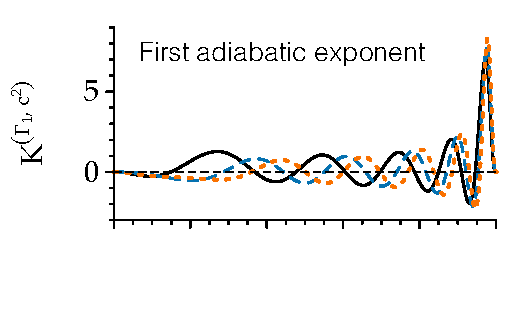
\includegraphics[width=0.5\textwidth,trim={0 1.1cm 0 0}, clip]{figs/pulse/kernels/kernel-ell-Gamma1_c2-diffusion.pdf}%
    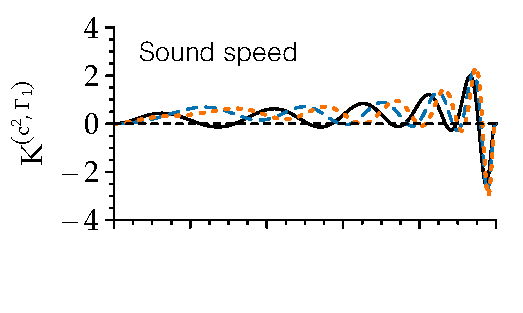
\includegraphics[width=0.5\textwidth,trim={0 1.1cm 0 0}, clip]{figs/pulse/kernels/kernel-ell-c2_Gamma1-diffusion.pdf}\\
    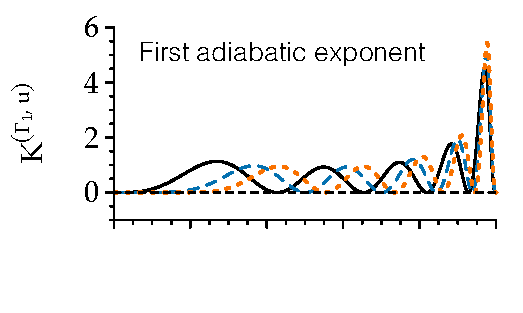
\includegraphics[width=0.5\textwidth,trim={0 1.1cm 0 0}, clip]{figs/pulse/kernels/kernel-ell-Gamma1_u-diffusion.pdf}%
    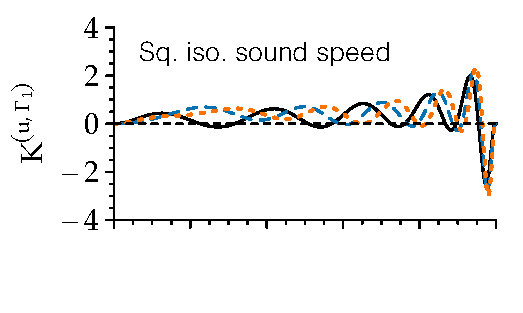
\includegraphics[width=0.5\textwidth,trim={0 1.1cm 0 0}, clip]{figs/pulse/kernels/kernel-ell-u_Gamma1-diffusion.pdf}\\
    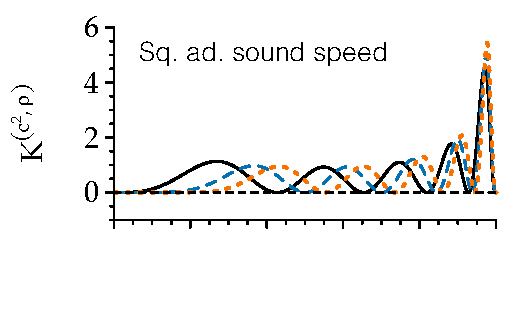
\includegraphics[width=0.5\textwidth,trim={0 1.1cm 0 0}, clip]{figs/pulse/kernels/kernel-ell-c2_rho-diffusion.pdf}%
    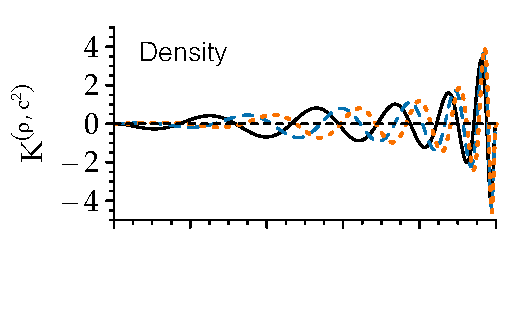
\includegraphics[width=0.5\textwidth,trim={0 1.1cm 0 0}, clip]{figs/pulse/kernels/kernel-ell-rho_c2-diffusion.pdf}\\
    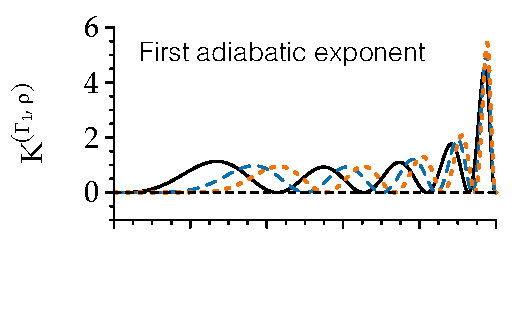
\includegraphics[width=0.5\textwidth,trim={0 1.1cm 0 0}, clip]{figs/pulse/kernels/kernel-ell-Gamma1_rho-diffusion.pdf}%
    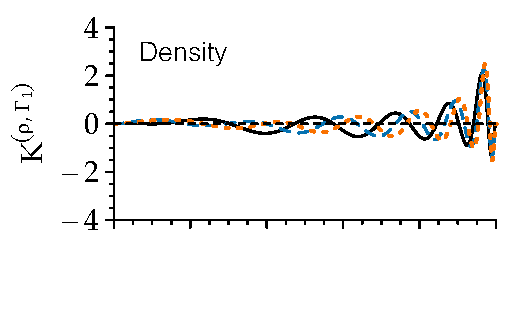
\includegraphics[width=0.5\textwidth,trim={0 1.1cm 0 0}, clip]{figs/pulse/kernels/kernel-ell-rho_Gamma1-diffusion.pdf}\\
    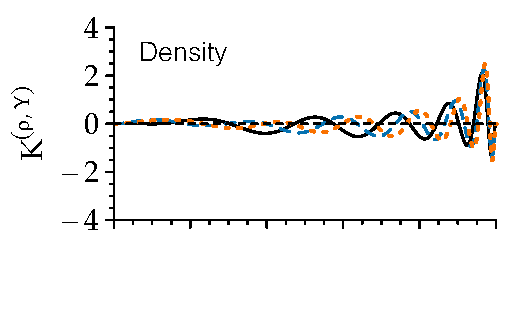
\includegraphics[width=0.5\textwidth,trim={0 1.1cm 0 0}, clip]{figs/pulse/kernels/kernel-ell-rho_Y-diffusion.pdf}%
    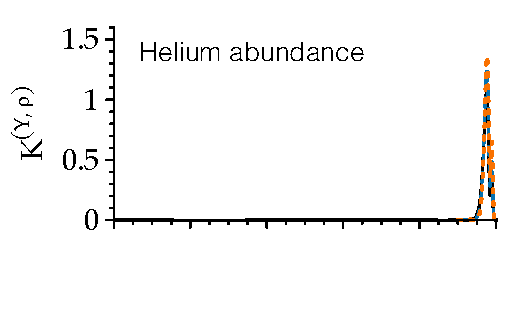
\includegraphics[width=0.5\textwidth,trim={0 1.1cm 0 0}, clip]{figs/pulse/kernels/kernel-ell-Y_rho-diffusion.pdf}\\
    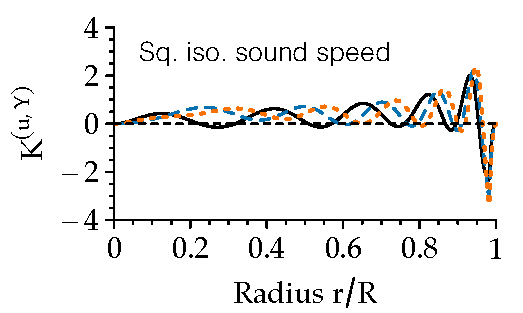
\includegraphics[width=0.5\textwidth]{figs/pulse/kernels/kernel-ell-u_Y-diffusion.pdf}%
    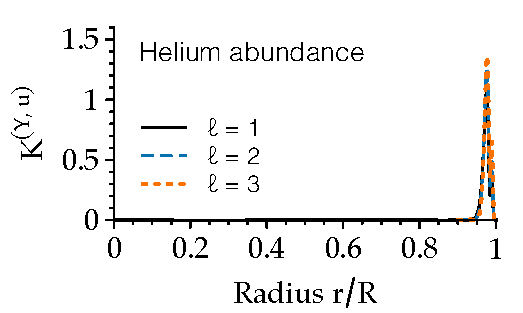
\includegraphics[width=0.5\textwidth]{figs/pulse/kernels/kernel-ell-Y_u-diffusion.pdf}
    \caption[Kernel functions (same $n$, different $\ell$)]{Pairs of kernel functions for modes with the same radial order ${n=5}$ and different spherical degrees ${\ell=1},2,3$. \label{fig:same-n}}
\end{figure}%
\begin{figure}
    \centering
    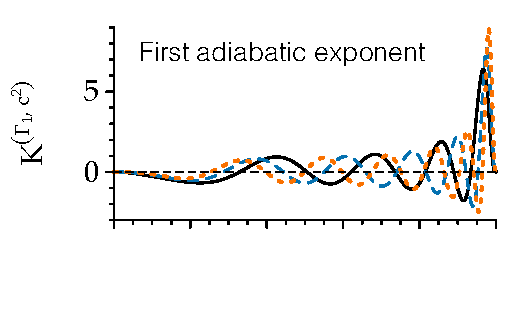
\includegraphics[width=0.5\textwidth,trim={0 1.1cm 0 0}, clip]{figs/pulse/kernels/kernel-n-Gamma1_c2-diffusion.pdf}%
    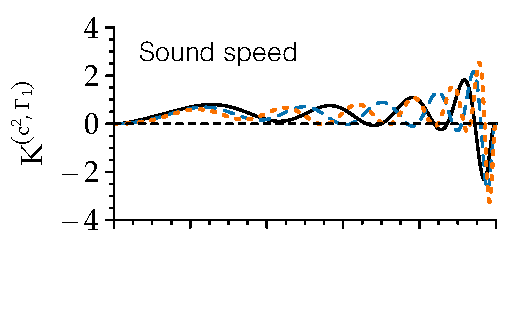
\includegraphics[width=0.5\textwidth,trim={0 1.1cm 0 0}, clip]{figs/pulse/kernels/kernel-n-c2_Gamma1-diffusion.pdf}\\
    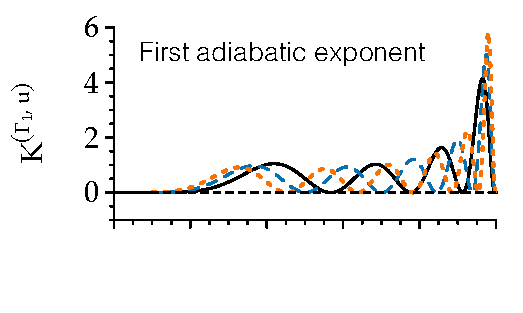
\includegraphics[width=0.5\textwidth,trim={0 1.1cm 0 0}, clip]{figs/pulse/kernels/kernel-n-Gamma1_u-diffusion.pdf}%
    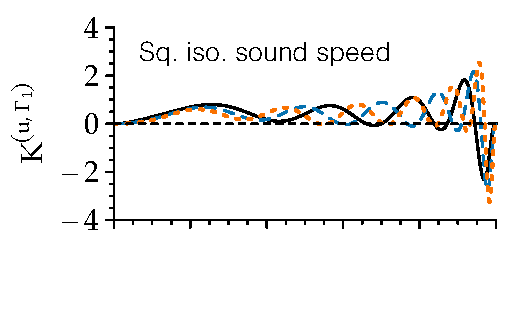
\includegraphics[width=0.5\textwidth,trim={0 1.1cm 0 0}, clip]{figs/pulse/kernels/kernel-n-u_Gamma1-diffusion.pdf}\\
    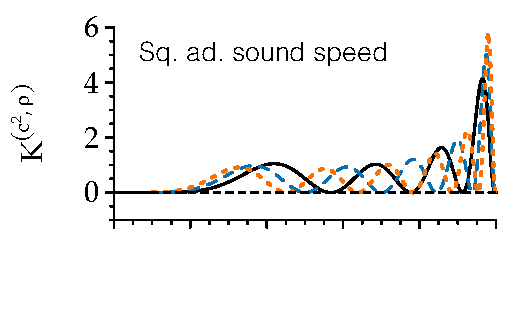
\includegraphics[width=0.5\textwidth,trim={0 1.1cm 0 0}, clip]{figs/pulse/kernels/kernel-n-c2_rho-diffusion.pdf}%
    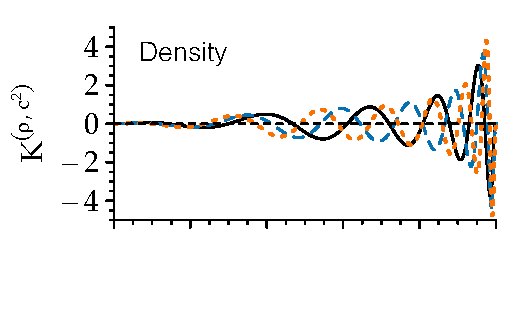
\includegraphics[width=0.5\textwidth,trim={0 1.1cm 0 0}, clip]{figs/pulse/kernels/kernel-n-rho_c2-diffusion.pdf}\\
    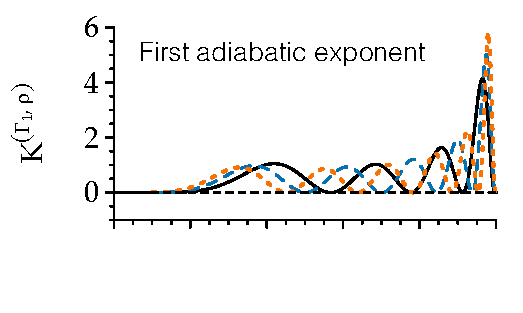
\includegraphics[width=0.5\textwidth,trim={0 1.1cm 0 0}, clip]{figs/pulse/kernels/kernel-n-Gamma1_rho-diffusion.pdf}%
    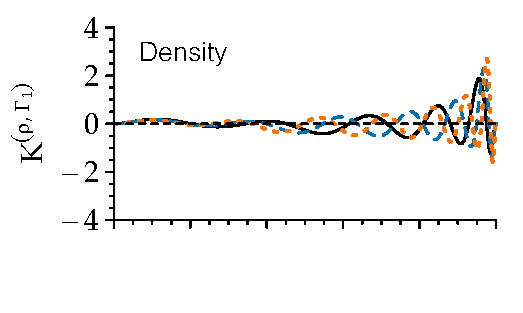
\includegraphics[width=0.5\textwidth,trim={0 1.1cm 0 0}, clip]{figs/pulse/kernels/kernel-n-rho_Gamma1-diffusion.pdf}\\
    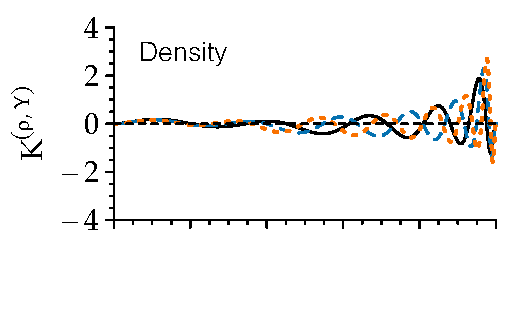
\includegraphics[width=0.5\textwidth,trim={0 1.1cm 0 0}, clip]{figs/pulse/kernels/kernel-n-rho_Y-diffusion.pdf}%
    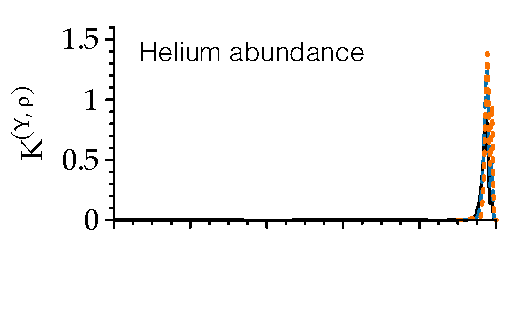
\includegraphics[width=0.5\textwidth,trim={0 1.1cm 0 0}, clip]{figs/pulse/kernels/kernel-n-Y_rho-diffusion.pdf}\\
    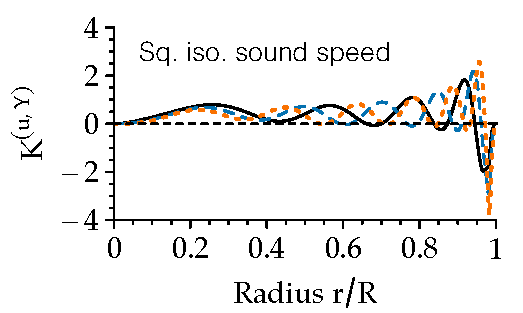
\includegraphics[width=0.5\textwidth]{figs/pulse/kernels/kernel-n-u_Y-diffusion.pdf}%
    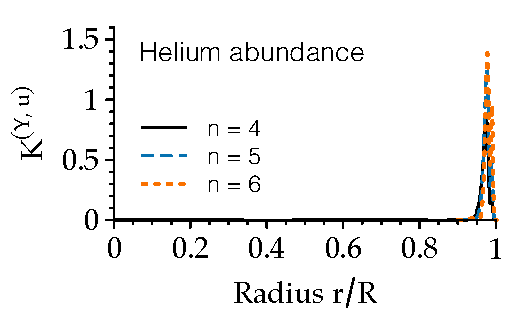
\includegraphics[width=0.5\textwidth]{figs/pulse/kernels/kernel-n-Y_u-diffusion.pdf}
    \caption[Kernel functions (same $\ell$, different $n$)]{Pairs of kernel functions for modes with the same spherical degree ${\ell=2}$ and different radial order ${n=4},5,6$. \label{fig:same-ell}}
\end{figure}%
%    }%
%}

\subsubsection*{Kernel Pair \texorpdfstring{$\mathbf{(\Gamma_1, \rho)}$}{(Gamma1,rho)}}
\noindent
Kernel functions for the first adiabatic exponent and density may be transformed from ${(c^2, \rho)}$ kernels via \citep[e.g.][Equations~104-105]{InversionKit}:
\begin{align}
    \KGr ={} & \Kcsr
\\  \KrG ={} & \Krcs - \Kcsr + \frac{G m \rho}{r^2} \int_{s=0}^r \frac{\Gamma_1 \chi^2 s^2}{2 \mathcal{S} \omega^2} \; \text{d}s
\\\notag   &+ \rho r^2 \int_{s=r}^R \frac{4\pi G \rho}{s^2} \left( \int_{t=0}^s \frac{\Gamma_1 \chi^2 t^2}{2 \mathcal{S} \omega^2} \; \text{d}t \right) \; \text{d}s.
\end{align}

\iffalse
\subsubsection*{Kernel Pair \texorpdfstring{$\mathbf{(\Gamma_1, c^2)}$}{(Gamma1,c2)}}
\begin{align}
    \KGcs &= P \cdot \ddr \left( \frac{\psi}{P} \right)
\\  \KcsG &= \Kcsr-\KGcs
\end{align}    
\fi

\subsubsection*{Kernel Pair $\mathbf{(u,Y)}$}
\noindent
Using additional assumptions, for example under assumption of the EOS, we may formulate kernels for other quantities such as the fractional helium abundance. 
For each mode $i$ we wish to obtain the pair of kernel functions for the isothermal sound speed (recall Equation~\ref{eq:speed-of-sound}) and helium abundance $Y$
\begin{equation}
    \vec K^{(2)}_i = \left[ \KuYnop, \KYunop \right]
\end{equation}
via conversion from the kernel pair of ${(\Gamma_1, \rho)}$
\begin{equation}
    \vec K^{(1)}_i = \left[ \KrG, \KGr \right].
\end{equation}
%In order to calculate the difference in helium abundance, we will need to assume an equation of state. 
We can expand the perturbation to the first adiabatic exponent as
\begin{equation}
    \frac{\delta \Gamma_1}{\Gamma_1}
    =
    \Gr \frac{\delta\rho}{\rho}
    +
    \GP \frac{\delta P}{P}
    +
    \GY \delta Y
\end{equation}
where I have introduced the quantities
%The calculations will therefore depend on the following variables that we may obtain from our reference model:
\begin{equation}
    \Gr \equiv \left( \pdv{\ln \Gamma_1}{\ln \rho} \right)_{P, Y} \qquad 
    \GP \equiv \left( \pdv{\ln \Gamma_1}{\ln P} \right)_{\rho, Y} \qquad
    \GY \equiv \left( \pdv{\ln \Gamma_1}{Y} \right)_{\rho, P}
\end{equation} 
which are calculated from the assumed EOS. 
There are two formulations of these kernels that appear in the literature: the \citet{ThompsonJCD2002} formulation and the \citet{Kosovichev1999} formulation. 
For the sake of completeness, I show both here. 

\begin{description}
\setlength{\itemindent}{0pt}
\item[Thompson--JCD Formulation.]
This kernel pair may be calculated with \citep[][their Equation~A9]{ThompsonJCD2002} 
\begin{align}
    \KYunop &= \GY \cdot \KGr
\\  \KuYnop &= \GP \cdot \KGr - P \cdot \ddr \left( \frac{\psi_i}{P} \right) \label{eq:Gough-JCD-KuY}
\end{align}
where ${\psi(r)}$ is the solution to the system of differential equations %(ibid.\ Equation~A5)
\begin{equation} \label{eq:bvp}
    \frac{\rho}{r^2 P}
    \psi_i
    =
    \frac{1}{4\pi G} \cdot %\left[
    \ddr \left( 
        \frac{F_i}{r^2 \rho} 
    %\right)
    -
    %\ddr \left( 
        \frac{1}{r^2 \rho} \cdot \ddra{\psi_i} 
    \right)
    %\right]
    %\ddr \left[ \frac{1}{r^2 \rho} \cdot \ddra{\psi_i} \right]
    %+
    %\frac{4\pi G \rho}{r^2 P} \psi
    %=
    %\ddr \left[ \frac{F_i}{r^2 \rho} \right]
\end{equation}
\begin{equation}
    F_i(r) = (\GP + \Gr) \cdot \KGr + \KrG
\end{equation}
with boundary conditions
\begin{equation} \label{eq:bcs1}
    \psi(r=0) = \psi(r=R) = 0.
\end{equation}
In order to calculate these kernels, we must first solve Equation~(\ref{eq:bvp}) for $\psi$ numerically. As it is a system of second-order differential equations, we must first massage it into a first-order system. We may integrate both sides of Equation~(\ref{eq:bvp}) to obtain 
\begin{equation}
    \ddra{\psi_i} = F_i - 4\pi G r^2 \rho \int_{s=r}^R \frac{\rho}{s^2 P} \psi_i \; \text{d}s.
\end{equation}
I use this approach here in this thesis. 
%After solving this equation, we may inspect the resulting $(u, Y)$ kernel pair. As with the $(c^2,\rho)$ kernels, Figures \ref{fig:same-n} and \ref{fig:same-ell} show these kernels for fixed radial order and fixed spherical degree, respectively. 


\item[Kosovichev Formulation.]
First let \citep[][his Equations~40; 43-45; 48]{Kosovichev1999}
\begin{equation}
    U = \U \qquad V = \VV
\end{equation}
\begin{align}
A &= \left(
  \begin{bmatrix} 
    V & -V \\
    0 & -U
  \end{bmatrix} 
  +
  \begin{bmatrix} 
    -V & 0 \\
    U & 0
  \end{bmatrix} 
  \begin{bmatrix} 
    1 & 0 \\
    -\Gr & 1
  \end{bmatrix}^{-1}
  \begin{bmatrix} 
    1 & 0 \\
    \GP & 0
  \end{bmatrix} \right)
= \begin{bmatrix}
    0 & -U \\
    V & U
  \end{bmatrix} \\
B &= \left(
  \begin{bmatrix}
    -V & 0 \\
    U & 0
  \end{bmatrix}
  \begin{bmatrix}
    1 & 0 \\
    -\Gr & 1
  \end{bmatrix}^{-1}
  \begin{bmatrix}
    -1 & 0 \\
    0 & \GY
  \end{bmatrix} \right)
= \begin{bmatrix}
    V & 0 \\
    -U & 0
  \end{bmatrix} \\
C &= \left(
  \begin{bmatrix} 
    1 & 0 \\
    -\Gr & 1
  \end{bmatrix}^{-1}
  \begin{bmatrix} 
    1 & 0 \\
    -\GP & 0
  \end{bmatrix} \right) 
= \begin{bmatrix}
    1 & 0 \\
    \Gr + \GP & 0
  \end{bmatrix} \\
D &= \left(
  \begin{bmatrix}
    1 & 0 \\
    -\Gr & 1
  \end{bmatrix}^{-1}
  \begin{bmatrix}
    -1 & 0 \\
    0 & \GY
  \end{bmatrix} \right)
= \begin{bmatrix}
    -1 & 0 \\
    -\Gr & \GY
  \end{bmatrix}.
\end{align}
%We have the kernels expressed in vector form %(ibid.\ Equation~34)
The kernels can be expressed in matrix form
\begin{equation} \label{eq:vec-k}
    \vec K^{(2)}_i = D^T \vec K^{(1)} - B^T \vec w
\end{equation}
with $\vec w$ being the solution of the differential equation %(ibid.\ Equation~33)
\begin{equation} \label{eq:vec-w}
    \ddx \left[ \vec w \right] = -A^T \vec w - C^T \vec K^{(1)}
\end{equation}
having boundary conditions %(ibid.\ Equation~28)
\begin{equation} \label{eq:bvs2}
    \frac{\delta \rho}{\rho} w_1 + \frac{\delta m}{m} w_2 = 0 \text{ at } r=0 \text{ and } r=R.
\end{equation}
By substitution of these matrices, we have that $\vec w$ is the solution to 
\begin{align}
    \ddxa{w_1} &= -\U w_2 - \KrG - \left( \Gr + \GP \right) \KGr \\
    \ddxa{w_2} &= \VV w_1 + \U w_2.
\end{align}
Since these derivatives are with respect to a logarithmic quantity, and recalling the identity
\begin{equation}
    \frac{\text{d}x}{\text{d}\ln y} = y\frac{\text{d}x}{\text{d}y} %\qquad \forall x,y \in \mathbb{R}
\end{equation}
we cast Equation~(\ref{eq:vec-w}) into a useful form as a linear system of first-order differential equations 
\begin{align}
    \ddra{w_1} &= -\frac{4\pi\rho r^2}{m} w_2 - \frac{1}{r} \left[ \KrG + \left( \Gr + \GP \right) \KGr \right] \\
    \ddra{w_2} &= \frac{G m \rho}{r^2P} w_1 + \frac{4\pi\rho r^2}{m} w_2
\end{align}
with the boundary conditions of Equation~(\ref{eq:bvs2}), which without loss of generality may be transformed into
\begin{equation} \label{eq:bvs}
    w_1(r = 0) = w_2(r=R) = 0.
\end{equation}
Finally we may calculate the kernels using this $\vec w$ by substituting the matrices above into Equation~(\ref{eq:vec-k}) to get
\begin{align}
    \KuYnop &= -\KrG - \Gr \cdot \KGr + \VV w_1 - \U w_2 \\
    \KYunop &= \GY \cdot \KGr.
\end{align}
%\emph{\textbf{TODO}: include some of Elliott's work (makes this easier to understand)}
\end{description}
These last kernels---the ${(u,Y)}$ kernel pair---are especially valuable for the following analysis. 
An inspection of their form (Figures~\ref{fig:same-n}~and~\ref{fig:same-ell}) reveals that the $Y$ kernels only have amplitude in ionization zones, which are located near to the stellar surface. 
As we will see later, this implies that it will be possible to isolate the effects of differences in mode frequencies to differences in internal isothermal sound speeds. 

%\newpage
\subsubsection*{Testing the Forward Formulation}

We may now compare the actual frequency differences between the two solar models to the differences that we get through the kernel equation (Equation~\ref{eq:forward}). 
The top pair of plots in Figure~\ref{fig:forward} shows this comparison for the ${(c^2, \rho)}$ and ${(u, Y)}$ kernel pairs. 
%Since I am interested in using this approach on asteroseismic data, 
Here I have shown the comparison using the set of modes (i.e., the ${n,\ell}$ labels) that have been observed in 16~Cyg~B. 
%Although the agreement is fairly good, the differences again increase as a function of frequency due to surface effects, as we have seen previously in Figure~\ref{fig:solar_freq_diffs}. 
As we have seen previously, the differences again increase as a function of frequency due to surface effects. 
We therefore modify Equation~(\ref{eq:forward}) to take this phenomenon into account by including the \citet{2014A&A...568A.123B} surface term: 
%The formulation becomes 
\begin{equation} \label{eq:forward-surf} \boxed{
  \frac{\delta\nu_i}{\nu_i} 
  = 
  \int_0^R \left[ K_i^{(f_1, f_2)} \frac{\delta f_1}{f_1}
                + K_i^{(f_2, f_1)} \frac{\delta f_2}{f_2}
          \right] \; \text{d}r
    + \frac{F(\nu_i)}{I_i}
}\end{equation}
where ${F(\nu_i)}$ is adapted from the surface term of Equation~(\ref{eq:BallGizon-surfterm})
\begin{equation}
    F(\nu_i) %= \frac{\delta \nu_i}{\nu_i}
    = 
    a_1 \left( \frac{\nu_i}{\nu_{ac}} \right)^{-2} + a_2 \left( \frac{\nu_i}{\nu_{ac}} \right)^{2}.
\end{equation}
%The bottom plots of Figure~\ref{fig:forward} show surface terms subtracted from the exact differences as well as the differences obtained through kernels. 
Figure~\ref{fig:forward} shows that after applying the surface term correction, the agreement between the exact differences and those obtained through the kernels is much better. 
In other words, through the use of the stellar structure kernels, we can translate differences in structure to differences in pulsation frequency. 

\begin{figure}
    %\begin{subfigure}[b]{0.5\linewidth}
        \centering
        \makebox[0.5\textwidth][c]{%
        \adjustbox{trim={0cm 1.1cm 0.3cm 0cm},clip}{%
            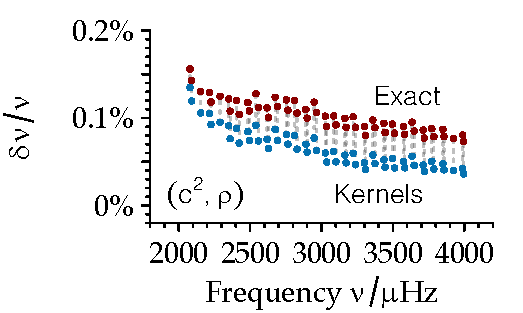
\includegraphics[width=0.5\textwidth]{figs/pulse/diffs/rel_diffs-c2_rho-D_no_diffusion.pdf}%
        }}\hspace*{-1cm}%
        %\includegraphics[width=\textwidth,keepaspectratio]{figs/pulse/diffs/rel_diffs_one_surfless-c2_rho-D_noD.pdf}
    %\end{subfigure}%
    %\begin{subfigure}[b]{0.5\linewidth}
    %    \centering
        \makebox[0.5\textwidth][c]{%
            \adjustbox{trim={2cm 1.1cm 0.3cm 0cm},clip}{%
                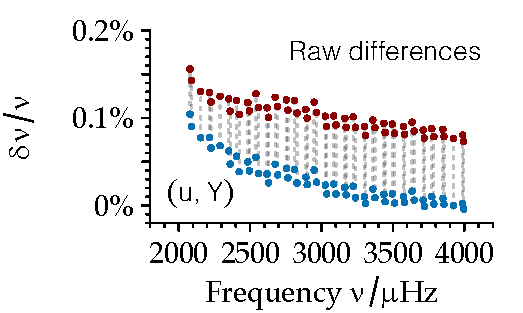
\includegraphics[width=0.5\textwidth]{figs/pulse/diffs/rel_diffs-u_Y-D_no_diffusion.pdf}%
            }}\\
        %\includegraphics[width=\textwidth,keepaspectratio]{figs/pulse/diffs/rel_diffs_one_surfless-u_Y-D_noD.pdf}
    %\end{subfigure}
    %\begin{subfigure}[b]{0.5\linewidth}
    %    \centering
        \makebox[0.5\textwidth][c]{%
            \adjustbox{trim={0cm 0cm 0.3cm 0cm},clip}{%
                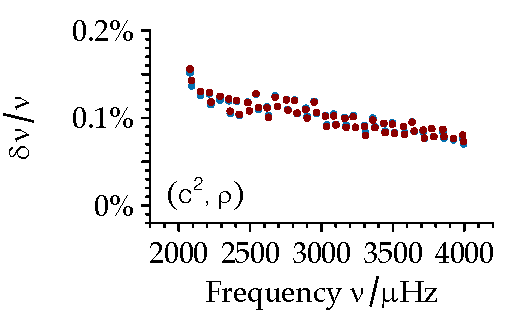
\includegraphics[width=0.5\textwidth]{figs/pulse/diffs/rel_diffs_surf-c2_rho-D_no_diffusion.pdf}%
            }}\hspace*{-1cm}%
        %\includegraphics[width=\textwidth,keepaspectratio]{figs/pulse/diffs/rel_diffs_one-c2_rho-D_noD.pdf}
    %\end{subfigure}%
    %\begin{subfigure}[b]{0.5\linewidth}
    %    \centering
        \makebox[0.5\textwidth][c]{%
            \adjustbox{trim={2cm 0cm 0.3cm 0cm},clip}{%
                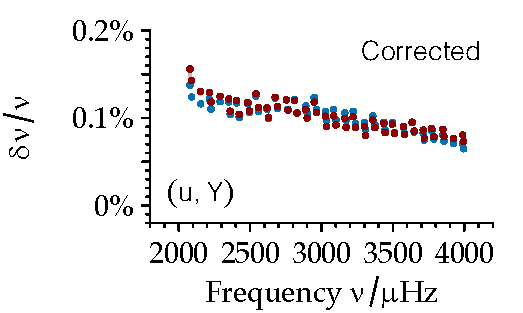
\includegraphics[width=0.5\textwidth]{figs/pulse/diffs/rel_diffs_surf-u_Y-D_no_diffusion.pdf}%
        }}
        %\includegraphics[width=\textwidth,keepaspectratio]{figs/pulse/diffs/rel_diffs_one-u_Y-D_noD.pdf}
    %\end{subfigure}
    \caption[Verifying the forward problem]{Top: Relative frequency differences between two solar models using the 16~Cyg~B mode set. 
    The points in red are the exact differences; the points in blue are the differences obtained through Equation~(\ref{eq:forward}) using ${(c^2, \rho)}$ kernels (left) and ${(u, Y)}$ kernels (right). 
    Bottom: the same, but also including the surface-term corrections of Equation~(\ref{eq:forward-surf}). 
    }
    \label{fig:forward}
\end{figure}


%\begin{figure}
%    \begin{subfigure}[b]{0.5\linewidth}
%        \centering
%        \includegraphics[width=\textwidth,keepaspectratio]{rel_diffs_one-c2_rho-D_noD.pdf}
%    \end{subfigure}%
%    \begin{subfigure}[b]{0.5\linewidth}
%        \centering
%        \includegraphics[width=\textwidth,keepaspectratio]{rel_diffs_one-u_Y-D_noD.pdf}
%    \end{subfigure}
%    \caption{Relative frequency differences of low-degree oscillation modes as a function of frequency between two solar models. The points in red are the exact differences; the points in blue are the differences obtained through Eqn.~\ref{eq:forward-surf} using $(c^2, \rho)$ kernels (left) and $(u, Y)$ kernels (right).} 
%    \label{fig:forward} 
%\end{figure}

%There are other kernel pairs that we have not written out here. These include $(u, \Gamma_1)$, $(\rho, Y)$, and $(c^2, \Gamma_1)$. All of these kernel pairs can be derived via manipulations of the kernels that we have already seen. Figure~\ref{fig:all-diffs} compares the exact differences between the non-diffusive and diffusive solar-calibrated models to the differences obtained through kernels. Being that the differences between the two are very small, this demonstrates that kernels are able to translate differences in structure to differences in frequency. 

%We will now turn our attention to going in the opposite direction---the \emph{inverse} problem---translating differences in frequency to differences in structure. 

\iffalse
\begin{figure}
    \centering
    \includegraphics[width=\textwidth,keepaspectratio]{figs/pulse/diffs/all_diffs-D_noD.pdf}
    \caption{Absolute differences between exact surface-term corrected relative frequency differences and surface-term corrected relative frequency differences obtained through the kernel equation (Equation~\ref{eq:forward-surf}) for six kernel pairs. \emph{\textbf{TODO}: remake figures} \label{fig:all-diffs} } 
\end{figure}
\fi


